\section{Mechanical Models II}
\label{MechModelsII:sec}

\subsection{Units}

ArtiSynth is primarily "unitless", in the sense that it does not
define default units for the fundamental physical quantities of time,
length, and mass associated with model components. Although time is
generally understood to be in seconds, and often declared as such in
method arguments and return values, there is no hard requirement that
it be interpreted as seconds. There are no assumptions at all
regarding length and mass. Some components may have default parameter
values that reflect a partcular choice of units, such as {\tt
MechModel}'s default gravity value of $(0, 0, -9.8)^T$ which is
associated with the MKS system, but these values can always be
overridden by the user.

Nevertheless, it is important, and up to the application developer to
ensure, that units be {\it consistent}. For example, if one decides to
switch length units from meters to centermeters (a common choice),
then all units involving length will have to be scaled appropriately.
Density, whose fundamental units ar3 $m/d^3$, where $m$ is mass and
$d$ is distance, needs to be scaled by $1/100^3$, or $0.000001$, when
converting from meters to centermeters.

Table \ref{Units:tab} lists a number of common physical quantities
used in ArtiSynth, along with their fundamental units expressed in
terms of mass ($m$), distance ($d$), and time ($s$).

\begin{table}
\begin{center}
\begin{tabular}{|lll|}
\hline
unit & fundamental units & \\
\hline
time                    & $s$ & \\
distance                & $d$ & \\
mass                    & $m$ & \\
velocity                & $d/s$ & \\
acceleration            & $d/s^2$ & \\
force                   & $m d/s^2$ & \\
work/energy             & $m d^2/s^2$& \\
torque                  & $m d^2/s^2$ & same as energy, somewhat counterintuitive \\
angular velocity        & $1/s$ & \\
angular acceleration    & $1/s^2$ & \\
rotational inertia      & $m d^2$ & \\
pressure                & $m/(d s^2)$ & \\
Young's modulus         & $m/(d s^2)$ & \\
Poisson's ratio         & 1 & no units; it is a ratio \\
density                 & $m/d^3$ & \\
linear stiffness        & $m/s^2$ & \\
linear damping          & $m/s$ & \\
rotary stiffness        & $m d^2/s^2$ & same as torque \\
rotary damping          & $m d^2/s$ & \\
mass damping            & $1/s$ & used in FemModel \\
stiffness damping       & $s$ & used in FemModel \\
\hline
\end{tabular}
\end{center}
\label{Units:tab}
\end{table}

\subsubsection{Scaling units}

For convenience, many ArtiSynth components, including {\tt MechModel},
implement the interafce
\javaclass[artisynth.core.util]{ScalableUnits}, which
provides the following methods for scaling mass and distance units:
%
\begin{lstlisting}
  scaleDistance (s);    // scale distance units by s
  scaleMass (s);        // scale mass units by s
\end{lstlisting}
%
A call to one of these methods should cause all physical quantities
within the component (and its descendents) to be
scaled as required by the fundamental unit relationships such
as shown in Table \ref{Units:tab}.

Converting a {\tt MechModel} from meters to centimeters can therefore be
easily done by calling 
%
\begin{lstlisting}
   mech.scaleDistance (100);
\end{lstlisting}
%
and adding the following code fragment to the end of the {\tt build()}
method in {\tt RigidBodySpring} (Section \ref{RigidBodySpringExample:sec})
%
\begin{lstlisting}
   System.out.println ("length=" + spring.getLength());
   System.out.println ("density=" + box.getDensity());
   System.out.println ("gravity=" + mech.getGravity());
   mech.scaleDistance (100);
   System.out.println ("");
   System.out.println ("scaled length=" + spring.getLength());
   System.out.println ("scaled density=" + box.getDensity());
   System.out.println ("scaled gravity=" + mech.getGravity());
\end{lstlisting}
%
will scale the distance by 100 and produce the following console output:
%
\begin{lstlisting}
   length=0.5
   density=20.0
   gravity=0.0 0.0 -9.8

   scaled length=50.0
   scaled density=2.0E-5
   scaled gravity=0.0 0.0 -980.0
\end{lstlisting}
%

It is important not to confuse scaling units with scaling
the geometry or mass itself. Scaling units should change
all physical quantities so that the simulated behavior of the
model remains unchanged.
If the distance-scaled version of {\tt RigidBodySpring} is
run, it should behave exactly the same as the non-distance
scaled version.

%\subsection{Multi-point springs}
%OPTIONAL
%\subsubsection{Operation}
%\subsubsection{Example: A single multi-point spring}

%\begin{figure}[h]
%\begin{center}
%\iflatexml
% 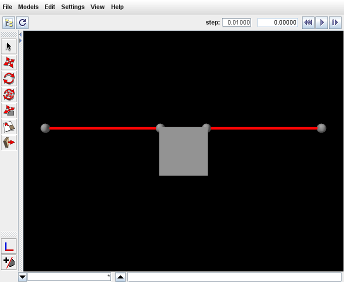
\includegraphics[]{images/MultiPointSpring}
%\else
% 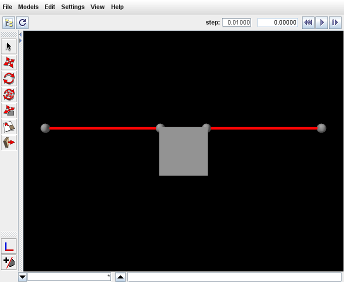
\includegraphics[width=3.75in]{images/MultiPointSpring}
%\fi
%\end{center}
%\caption{MultiPointSpring model loaded into ArtiSynth.}
%\label{MultiPointSpring:fig}
%\end{figure}
%
%A simple model showing a multi-point spring is defined in
%%
%\begin{verbatim}
%  artisynth.demos.tutorial.MultiPointSpring
%\end{verbatim}
%

% MultiPointSpring

\subsection{Point-to-point muscles}
\label{PointToPointMuscles:sec}

\subsubsection{Muscle materials}

\subsubsection{Example: Muscle attached to a rigid body}

\begin{figure}[h]
\begin{center}
\iflatexml
 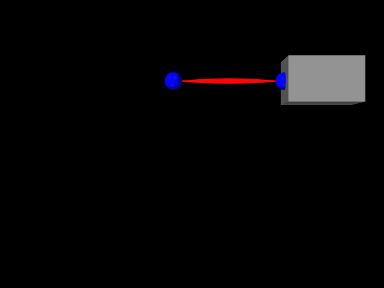
\includegraphics[]{images/SimpleMuscle}
\else
 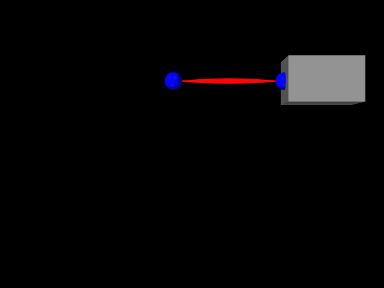
\includegraphics[width=3.75in]{images/SimpleMuscle}
\fi
\end{center}
\caption{SimpleMuscle model loaded into ArtiSynth.}
\label{SimpleMuscle:fig}
\end{figure}

A simple model showing a single muscle connected to a rigid
body is defined in
%
\begin{verbatim}
  artisynth.demos.tutorial.SimpleMuscle
\end{verbatim}
%

% SimpleMuscle

%\subsubsection{Multi-point muscles}

%\subsection{Mesh components}
%OPTIONAL 
%\subsubsection{Fixed meshes}
%\subsubsection{Simple mesh example}

% SimpleMesh

%\subsubsection{Skinned meshes}
%\subsubsection{Simple skinned mesh example}

% SimpleSkinnedMesh

\subsection{Collision Handling}

Collision handling in ArtiSynth is implemented by a collision
handling mechanism build into {\tt MechModel}. Collisions are
disabled by default, but can be enabled between rigid and deformable
bodies (finite element models in particular), and more generally
between any body that implements the interface 
\javaclass[artisynth.core.mechmodels]{Collidable}.

%\subsubsection{Collidable bodies}

\subsubsection{Enabling collisions in code}

Collisions can be enabled as either a default behavior between all
bodies, a default behavior between certain {\it types} of
bodies, or a specfic behavior between individual pairs of bodies.

The methods for controlling collision behavior include:
%
\begin{lstlisting}
  setDefaultCollisionBehavior (behavior);
  setDefaultCollisionBehavior (enabled, mu);
  setDefaultCollisionBehavior (typeA, typeB, behavior);
  setDefaultCollisionBehavior (typeA, typeB, enabled, mu);
  CollisionBehavior getDefaultCollisionBehavior (typeA, typeB);

  setCollisionBehavior (a, b, enabled, mu);
  setCollisionBehavior (a, b, behavior);
  CollisionBehavior getCollisionBehavior (a, b);
\end{lstlisting}
%

\subsubsection{Example: Collision with a plane}

\begin{figure}[h]
\begin{center}
\iflatexml
 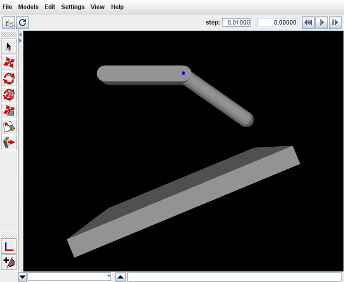
\includegraphics[]{images/JointedCollide}
\else
 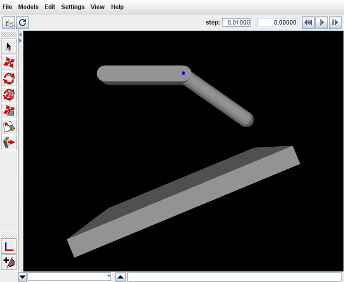
\includegraphics[width=3.75in]{images/JointedCollide}
\fi
\end{center}
\caption{JointedCollide model loaded into ArtiSynth.}
\label{JointedCollide:fig}
\end{figure}

A simple model illustrating collision between two jointed rigid bodies
and a plane is defined in
%
\begin{verbatim}
  artisynth.demos.tutorial.JointedCollide
\end{verbatim}
%

% JointedCollide

\subsubsection{implementation and limitations}

%\subsection{Moving non-dynamic components}

%\subsection{General component arrangements}
%\label{GeneralArrangements:sec}

%OPTIONAL

%\subsubsection{Component lists}

%\subsubsection{General arrangement example}

% NetDemo

%\subsubsection{Legacy containers in MechModel}

\subsection{Render properties}
\label{RenderProperties:sec}

\subsubsection{Render property taxonomy}

\subsubsection{Setting render properties}

\subsection{Scaling and transforming}

OPTIONAL

\subsubsection{The ScalableUnits interface}

\subsubsection{The TransformableGeometry interface}
